\subsection{The Frontend Software Stack}
In IoT embedded systems, you usually have three options for the front-end stack:
bare-metal, a real-time operating system (RTOS), or full operating system, like
Linux. In this context, "front-end" refers to the edge computing devices, and
"back-end" refers to the cloud services. For our project, Linux isn't an option
due to power constraints, which in turn affects processing power. Also, most
low-power microcontrollers, including some that include ARM Cortex M0 and M4
cores, don't have a memory management unit (MMU), which is required by the Linux
kernel. So, we are really left with two options: bare-metal or an RTOS. Before
discussing either choice, we first will discuss the software requirements for
the front-end. 

At its core, all the sensor nodes need to do is periodically take readings and
transmit them back over the LoRaWAN protocol to a gateway. Once it is received
by the gateway, the results are sent to our back-end service for additional
processing. The nodes should be able to receive commands over LoRaWAN to adjust
how often sensor readings should ideally take place, perform firmware updates,
or update the device's configuration. The device should be aware of its current
power constraints, such as the current battery level, the rate at which it's
charging, the rate at which it uses power, and whether it is plugged into USB
power. It should make decisions based on these characteristics, such as how
often to take sensor readings, and therefore, how long it should sleep for (and
the sleep mode). On the LoRa-E5, the device is equipped with a ARM Cortex-M4
microcontroller capable of sleep, deep-sleep, and standby low-power modes, each
have the ability to be woken up from the real-time clock (RTC) or specific I/O
pins. Any choice in choosing front-end software stack components should not
hinder the core's ability to move into either of these modes. Ideally, the
standby low-power mode is preferred since it offers the best power efficiency -
down to approximately 360nA. If the firmware deems that it cannot meet the
sensor reading frequency goal, it should communicate to the back-end about its
power deficit and inform the owner. It then will adjust the reading frequency to
stay as self-sustaining as possible. If the user wants to, they should be able
to disable this feature. Also, if the device is plugged in over USB, the device
doesn't need to go into sleep anymore since power is being provided through USB.
Also, if the device were asleep, then it wouldn't be able to respond to the user
through the command-line interface (CLI). Thus, if plugged-in, the device should
never go to sleep. As just mentioned, the device should provide a CLI interface
for configuration or view real-time sensor measurements. The software
requirements are shown below.


The device should be able to...
\begin{itemize}
	\item Enter the standby low-power mode
	\item Perform over-the-air firmware or configuration updates
	\item Be aware of its power constraints and budget, and adjust the
		frequency at which it takes sensor readings
	\item Periodically take sensor readings as the frequency specified by the
		user, if possible
	\item Reconfigure any of the sensors machine-learning models
	\item Be woken up when connected to a computer over USB
	\item Provide a CLI when connected over USB that allows for the device's
		configuration and real-time output of the sensor's data
\end{itemize}

% Maybe can make a GUI interface with Python?
% There can at least be a TUI for the CLI (client-side)
\subsubsection{Bare Metal Architecture}
A bare metal software architecture refers to programming the microcontroller
directly by modifying its registers or with its hardware abstraction layer
(HAL). With bare metal programming, there is no operating system involved. A
HAL provides facilities for controlling the microcontroller and accessing its
peripherals independent of the specific model, but only for the same vendor. The
other method of bare metal programming is through using the MCU's header files
that contain register definitions (addresses), and manually reading from and
writing to them. The architecture of a bare metal program typically includes an
initialization phase followed by an infinite loop. Inside the infinite loop,
registers might be polled and tasks can be done. The infinite loop can
essentially be a synchronous event loop. Asynchronous execution can only happen
through interrupt service routines (ISRs), or if the microcontroller has more
than one core. ISR handlers must be manually written for bare metal programming
to allow for asynchronous, non-blocking events to occur. ISRs are typically
written for direct memory access (DMA) controllers, analog to digital converters
(ADCs), I/O, such as \iic or pin interrupts, and much more. When an ISR occurs,
usually some kind of global variable is update to inform the event loop that
something has occurred. Bare metal programming is typically done when the
microcontroller doesn't have the processing power, or other peripherals, to run
an operating system. A bare metal program allows for the most amount of
determinism, which is important for for real-time systems. RTOSes try provide
some higher level abstractions while maintaining determinism. Another reason why
bare metal programming might be chosen over using an operating system is that
bare metal programming can provide the best performance for both compute and
memory usage.

\begin{figure}[h]
\centering
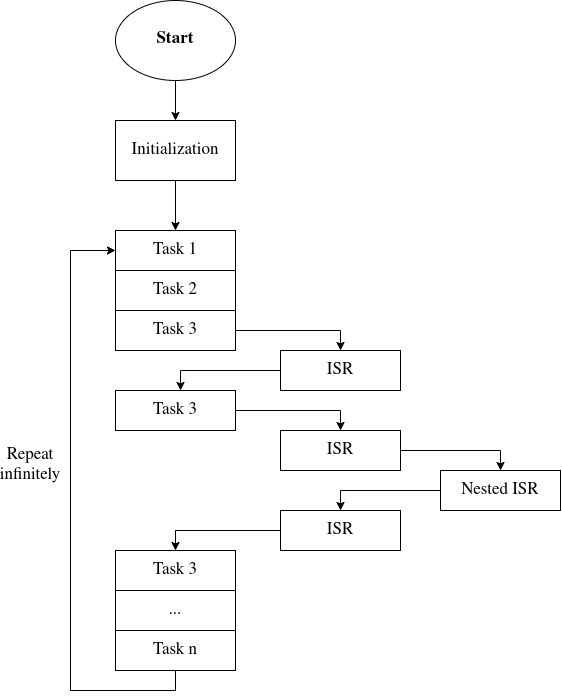
\includegraphics[width=3.25in]{bare-metal-arch.png}
\caption{Typical Bare Metal Embedded System Software Architecture}
\label{fig:bare-metal-arch}
\end{figure}

Figure \ref{fig:bare-metal-arch} depicts an example of the control flow a bare
metal program typically takes. On boot, the main function is executed. This is
followed by one or many initialization functions that configure the system for
the specific application. This usually involves configuring the clock speed, ADC
timings, DMA initialization, I/O pin direction and functionality, etc. Once the
initialization is complete, the main loop executes infinitely until either the
microcontroller hits an unhandled trap (error/exception) or is powered off. Each
task, task 1 through n, is completed synchronously. The task might poll a bit in
a register to see if, for example, an I/O transaction is complete, or it could
be performing a computation. The synchronous execution can only be interrupted
through an interrupt, assuming there is a enabled and linked ISR. In the figure,
task 3 is asynchronously interrupted twice. First, by a single-level interrupt.
And, second, by an interrupt that was then interrupted by an interrupt with a
higher priority than the one currently executing. In between the first and
second interrupt, task 3 was resumed, executed some more, and then paused again
for the second round of interrupts. When the CPU is interrupted, the state of
the CPU is saved onto the stack. When the ISR completes, the state is restored
and what was previously executing can as if nothing had changed.  However, this
can cause problems during critical sections of code. Usually, ISRs can be
disabled and deferred during the sections, or the code can be rethought.
Finally, after the second round of interrupts, task 3 completes and so does the
rest of the loop. The execution will repeat starting at task 1, but the
interrupts don't necessarily have to execute (as shown) at the same as the
previous loop. Interrupts can happened whenever.


\subsubsection{FreeRTOS Architecture}
FreeRTOS is an specific type of operating system that focuses on determinism and
predictability, rather than responsiveness, like in Linux, Mac OS X, or Windows.
It supports preemption and co-operative scheduling, as well as priority
inheritance to prevent priority inversion. FreeRTOS is small. It only requires 5
to 10 kB of RAM for operation. FreeRTOS, like many other RTOSes focuses mainly
on task scheduling and communication. In fact, the main source files provided
for FreeRTOS are:

\begin{itemize}
	\item tasks.c - for creating and managing task's priority and state
	\item queue.c - for task to task communication - also includes mutex and
		semaphors implemented with queues
	\item list.c - a generic linked-list implementation
	\item timers.c - timer implementation
	\item port.c - MCU specific code for porting FreeRTOS
	\item FreeRTOSConfig.h - FreeRTOS configuration
\end{itemize}

All of the data structures provided by FreeRTOS integrate with tasks and will
automatically block/un-block them, such as waiting for a timer or other event.
Code written for FreeRTOS can also be transferred to other microcontrollers that
are not necessarily from the same vendor. This is because of the layered
software abstraction architecture. At the lowest level, is bare metal
programming with a HAL. Above that, is MCU specific code to implement low-level
FreeRTOS code, called a port (\emph{port.c} as shown in the list above). On top
of the platform specific FreeRTOS port code is the platform independent FreeRTOS
code. This is the code that is responsibly for the main logic of FreeRTOS, such
as the kernel, queue and list data structures, and other middleware. The
user/programmer code is written above the platform independent FreeRTOS code.
This has many ramifications, such as what was already mentioned back code
portability. Since the FreeRTOS main interface is platform independent,
middleware can be more easily written in a standardized way, such as providing
support for FAT file systems, USB communication, LoRa/LoRaWAN, cryptography, and
much more.

At its core, FreeRTOS is all about scheduling tasks and communicating between
them. Most of the code is oriented around configuring and initializing tasks.
FreeRTOS is deterministic because of its scheduling algorithm. Generally, the
task with the highest priority should be running. A task with a priority of 0
has the lowest priority, like the idle task, and a task with priority
$configMAX\_PRIORITY - 1$ has the highest priority. The
\emph{configMAX\_PRIORITY} definition is a user defined parameter inside of
FreeRTOSConfig.h that defines how many priorities there are for scheduling. The
more priorities there are, the more memory the kernel will need since each
priority needs a list allocated for each task state. Priorities are manually
assigned by the programmer, so with knowledge of the scheduling algorithm (which
can be configured), the programmer can reason about potential issues much
easier. The scheduler can be configured to be preemptive or non-preemptive. With
non-preemptive scheduling, tasks must either block, suspend, or complete before
another task can be executed. Once a task is put into a not-running state, the
task with the highest priority is selected. If two tasks have the same priority,
they are selected using a round robin algorithm. Non-preemptive scheduling is
good if tasks are commonly executing critical sections of code, or using shared
resources.  However, this can lead to some tasks being starved and are not able
to make progress even though they have a higher priority than the task currently
running since it never blocks or suspends. Each task state is represented as an
array of lists where the index into the array represents the task's priority.
The number of priority levels is defined by the programmer in FreeRTOSConfig.h.
For example, when a task with priority 2 moves from the blocked to ready state,
the scheduler will find it in the blocked array at index 2. It'll then search
through the list that's at index 2 until it finds the task, and it'll move it to
the list in the ready array at index 2. Each time the scheduler executes, it'll
iterate through each list inside the ready array. Each task has a task control
block (TCB) to manage the task's state, like where its stack is located (start
and end addresses), its priority, its name, and pointers to list item objects so
that the list the task is in can be found quickly.

Figure \ref{fig:freertos-task-sm} shows the different states a task can be in
along with state transitions. The two main states are: running and not-running.
Not-running is a super state, which means it has sub-states. If a task is not
running, then it can be either suspended, blocked, or ready. A task that is
suspended is not available to the scheduler, and therefore cannot make progress
unless manually resumed by another task. Tasks can be put in the suspended list
from any other state, and can be done through the vTaskSuspend() function. When
vTaskResume() is called, a task is moved from the suspended state (list) to the
ready state (list). A blocked task is similar to a suspended task except that a
blocked tasks is available to the scheduler and can make progress once it is
unblocked. A task can be unblocked from many different kinds of events, such as
from a timer expiring, a specific interrupt triggering an event, the
availability of a semaphore, or the unlocking of a mutex. Before any task can be
executed, it must first be moved into the ready state. Whenever the scheduler
runs, either after each tick or when a running process stops running, it looks
in the ready list and looks for the highest task to run.

\begin{figure}[h]
\centering
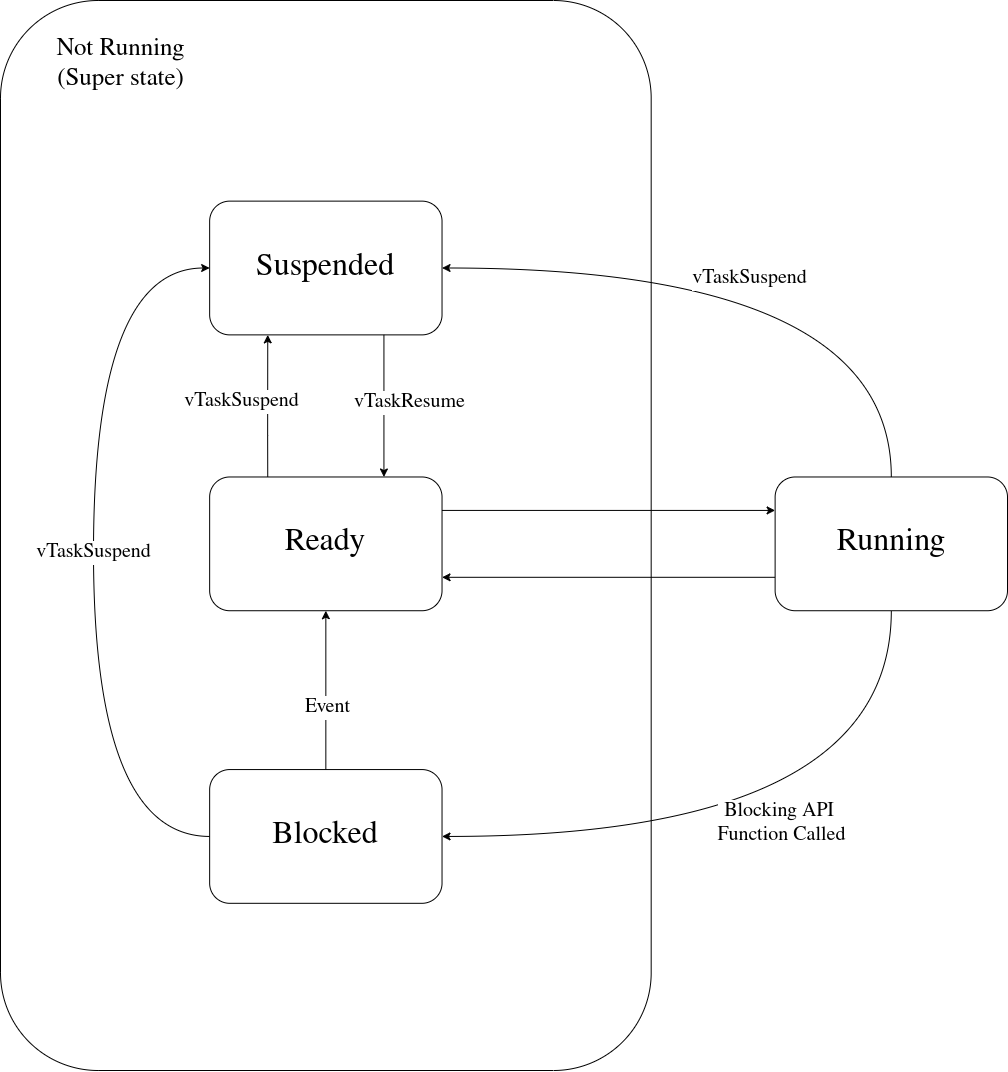
\includegraphics[width=3.25in]{freertos-task-sm.png}
\caption{The FreeRTOS Task State Machine}
\label{fig:freertos-task-sm}
\end{figure}

A preemptive scheduler interrupts tasks whether they want to be or not. A
preemptive scheduler interrupts tasks at a pre-defined interval, set in
FreeRTOSConfig.h, called a ``tick''. Preemption can also occur when a task with
a higher priority becomes ready for execution. At every tick, the scheduler will
set the tasks with the highest priority as the active task, choosing tasks with
an identical priority using a round-robin algorithm. Whenever there are no tasks
in the ready list, the idle tasks is executed. It has the lowest priority
level, 0. The idle tasks also allows the programmer to hook into it to execute a
handler each time the idle task is entered. The idle tasks performs maintenance,
such as cleaning up freed memory freed during the task execution. When a task
frees memory, that memory isn't actually removed from the heap until the idle
task is ran in order to keep user tasks deterministic. Figure
\ref{fig:freertos-tick-arch} shows an example of the execution of three tasks
each with different priorities. The vertical axis represents the task's
priority, while the horizontal axis represents time and how long tasks executed.
The kernel tasks and interrupts always have the highest priority, and are
depicted at the top in red. The kernel runs the scheduling algorithm each time a
task goes from running to not running, or on each tick assuming it is configured
to use preemption and tick-mode. In the figure, arrows are only added when the
scheduler/kernel runs and swaps the currently running task with another. Each
time there's a red bar, the kernel is running instead of a previously running
task, but arrows are not included so the diagram doesn't look too busy. Thin,
horizontal bars between tasks on the same priority represents that task moving
into the ready list, and is based on the task color. Initially, \emph{Task A}
is running, but it preempted by \emph{Task D} when it becomes unblocked due to
an asynchronous event at time \emph{t1}, such as a timer or a transaction is
received over \iic. At time \emph{t2}, \emph{Task D} is blocked, so the next
available task to run with the highest priority is selected, \emph{Task B}.
Since \emph{Task B} and \emph{Task C} share the same priority level, on the
second tick (time \emph{t3}), \emph{Task C} is ran since the scheduler tries to
be as fair as possible for tasks sharing priority.  Similarly, at time
\emph{t4}, \emph{Task C} is ran instead of \emph{Task B} since \emph{Task B} and
\emph{Task C} are the only tasks that share a priority of 2. At time \emph{t5},
\emph{Task B} is blocked, so \emph{Task A} is ran since has the highest priority
level of all ready tasks.  Next, at time \emph{t6}, \emph{Task A} is blocked or
suspended, and since there are no ready tasks, the idle task is ran. Finally, at
time \emph{t7}, \emph{Task D} is moved into the ready state, and the scheduler
starts executing it.

\begin{figure}[h]
\centering
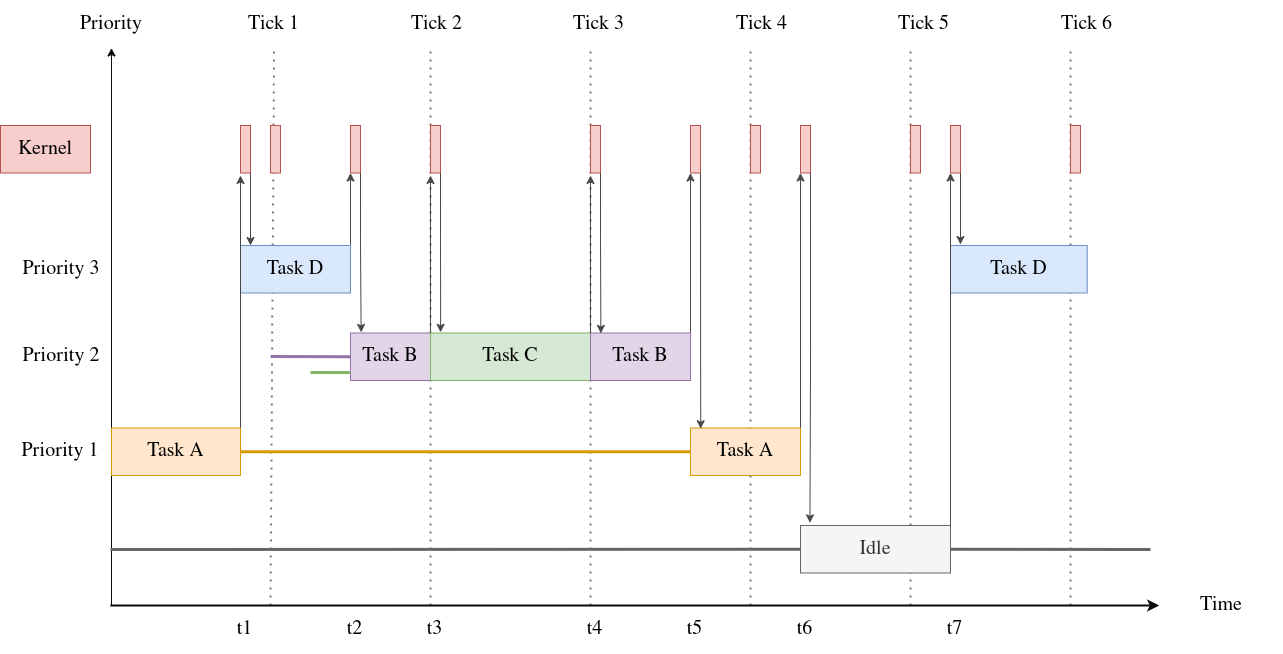
\includegraphics[width=4.25in]{freertos-tick-arch.png}
\caption{FreeRTOS Preemptive Execution}
\label{fig:freertos-tick-arch}
\end{figure}

However, preemptive scheduling can cause synchronization issues for accessing
shared resources.  Consider the following example: two tasks, task A and task B,
have the same priority and want to transmit strings over same UART channel, the
shared resource. Task A wants to send "abcdefghi" and task B wants to send
"123456".  However, the example would still work if task B had a higher priority
than task A, task B is blocked or suspended initially while task A is running.
At tick, t$_0$, task A is running and starts sending its message. At tick,
t$_1$, since task A and task B have an identical priority, task B is swapped
with task A.  But, at t$_1$, task A was only able to send "abcd". Now, consider
just for the example, that task B is able to send the entirety of its message,
"123456". At this point in time, "abcd123456" has been transmitted over UART.
Finally, at tick t$_3$, task A is able to complete sending its message by
sending the remainder, "efghi". The end result is that "abcd123456efghi" was
transmitted over UART. The message was corrupted. 

Luckily, FreeRTOS, like other operating systems, provide utilities for
synchronizing asynchronous operations: mutexes and semaphors. While similar,
they are used for vastly different scenarios.  Mutexes act as keys for locked
doors. Only one person, or process/task, can hold onto the key at the same time
- they are binary. Mutexes are used for synchronizing access to shared
resources. For each resource, akin to having multiple locked doors, requires an
unique mutex, or key, to gain permission to access it. Semaphors, while similar
in implementation to mutexes as they can be explained as non-binary mutexes,
their purpose is vastly different. Semaphors are meant for signalling events.
The key difference here is that with semaphors, there is a producer and
consumer, and they don't need to be the same task/process. Whereas with mutexes,
only the task that holds the mutex can release it. A problem with using
semaphors as mutexes is that a semaphore doesn't portray which resource has been
taken. Say there are two UART channels and two tasks. If a semaphore were used
to allocate one of the UART channels, then the other task wouldn't know which
UART channel is available. In order to portray that, state variables would need
to be introduced, but this can cause more errors. It's better, for any kind of
resource allocation and synchronization, to use unique mutexes for each. All
sources used in this subsection comes from the FreeRTOS reference manual
\cite{freertos-ref}, the FreeRTOS tutorial guide \cite{freertos-guide}, and
a breakdown of the FreeRTOS internal architecture \cite{about-freertos-arch}.

An issue that arises in RTOSes, and operating systems in general, when using
synchronization mechanisms is priority inversion. Priority inversion is a
situation where a lower priority task effectively has higher priority than
another task that was originally defined with a higher priority. It is more
clear through the use of an example. Consider three tasks, \emph{A}, \emph{B},
and \emph{C}, with priorities 1, 2, and 3, respectively. Tasks \emph{A} and
\emph{C} share a resource that uses a mutex to synchronization. Consider, that
initially task \emph{A} is executing before \emph{C}, and grabs onto the mutex.
Then, some time later, task \emph{C} is unblocked and begins executing and wants
to use the shared resource, so it tries to grab onto the mutex. The mutex
already belongs to task \emph{A}, so now task \emph{C} must wait and block.
After \emph{C} starts to block, task \emph{B} begins to execute. If task
\emph{A} was previously executing, which it would've since it took the mutex for
\emph{a reason}, task \emph{B} would have preempted it. Now, as long as \emph{B}
is executing and \emph{A} holds the mutex, then \emph{C} cannot make progress
even though it technically should be since it has higher priority. The only
thing keeping it from executing is the execution speed of task \emph{A} and how
much processing it does while holding onto the mutex. Thus, effectively, the
priorities between task \emph{B} and \emph{C} have been swapped.

The solution to priority inversion is priority inheritance. Priority inheritance
is where two tasks share a resource guarded by a mutex, and the task with the
highest priority will share its priority with the lower priority task so that
the higher priority task can make progress as soon as possible. The higher
priority task might be performing safety critical or just critical sections of
code, so it's important that they preempt lower priority tasks or let them
finish as soon as possible if they hold mutexes. FreeRTOS implements priority
inheritance by adding a pointer field, pxMutexHolder, which holds a pointer to
the task that currently owns the mutex. If a task with a higher priority is
waiting on the mutex, then it'll check pxMutexHolder, and if pxMutexHolder
points to a task that has a lower priority, then the FreeRTOS scheduler/kernel
will let it inherit the other task's priority.

Lastly, one of FreeRTOS's features that would be of interest for this project is
its tick-less operation mode. As previously mentioned, tick-less modes allow the
tick interrupt to be disabled to allow the device to go into a deep sleep. This
is needed for the MCU to go into deep sleep because the tick interrupt would
wake up the system, and any currently running tasks that depend on timers would
be disrupted. Tick-less mode can be enabling tick-less idle in the FreeRTOS
configuration file. The tick-less idle mode will automatically be entered when
the following conditions are met:

\begin{enumerate}
	\item The idle task is the only task able to run because all other tasks are
		in the \emph{blocked} or \emph{suspended} state
	\item The idle tasks is expected to be executed for n or more complete ticks,
		where n is a user configured value called
		\texttt{configEXPECTED\_IDLE\_TIME\_BEFORE\_SLEEP}
\end{enumerate}

\subsubsection{Architecture Deliberation}
One of the main considerations in choosing parts and in making software
architecture decisions is power efficiency. A bare-metal architecture would
give us the ultimate control in how the microcontroller behaves at the cost of
flexibly, code re-use, code maintainability, and time required to build a
complete prototype. A bare-metal architecture typically involves a main loop
that polls various register values until certain conditions (application
specific) are met, does a few actions, then repeats. Interrupt service routines
(ISRs) are written specifically for that application. If more functionality
needs to be added, it could touch every piece of the bare-metal architecture.
These lead to more complicated implementations that don't tend to scale well.
Adding a `simple' feature could end up requiring a complete re-write of the
application.  

For simple applications, a bare-metal architecture is perfect.
However, if there are lots of asynchronous events, such as I/O, it becomes more
difficult to maintain. Also, by using a RTOS, it allows the programmer to use
middleware, such as a FAT file system driver. So, ideally, we would like to use
a RTOS, specifically FreeRTOS since it is officially supported by STM. However,
RTOSes maintain time by interrupting the system at a set frequency, or a tick,
to do job control and other maintenance.  This tick-architecture prevents the
microcontroller from going into sleep since the RTOS needs it to maintain time
for process timers. Luckily, FreeRTOS has a tick-less mode which allows the
device to go into deep-sleep and standby mode. Therefore, since we need to deal
with both USB and LoRa communication, as well as other asynchronous
communication with the sensors, we chose to go with FreeRTOS for the main part
of the front-end stack. 

The middleware provided for free for the LoRa-E5 is the
following: FatFS, FreeRTOS, LoRaWAN, KMS (key management service), cURL,
mbed-crypto (cryptographic services). For the sensor nodes, we will be using
FreeRTOS, LoRaWAN, FatFS for training the sensor ML models, STM FUOTA (Firmware
Update Over The Air) and mbed-crypto for securely transmitting data over LoRa.

% \subsubsection{Middleware}
